\documentclass{article}
\usepackage[english]{babel}
\usepackage{graphicx}
\usepackage{tabularx}

\title{Electromagnetic Inverse Design}
\author{Jesse Lu and Jelena Vuckovic}
\date{SPRC 2009 Symposium}

\begin{document}
\maketitle % put the title in
\thispagestyle{empty} % this removes page numbers
\noindent\makebox[\textwidth]{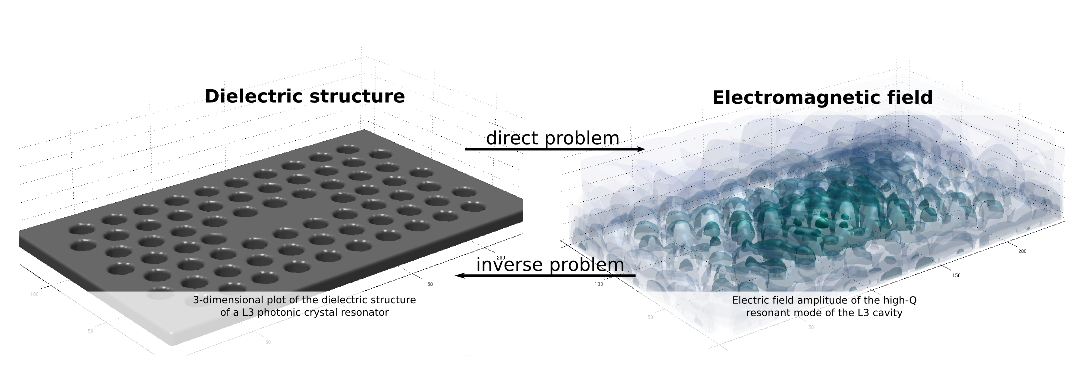
\includegraphics[width=1.6\textwidth]{fig1}}% this is fancy stuff to make a centered, but very wide picture

We develop a method to solve the electromagnetic inverse design problem; that is, to find a dielectric structure that will produce a specified electromagnetic field. Such a method enables the design of non-intuitive, multi-objective photonic components such as small mode-volume or doubly-resonant cavities, broadband waveguide couplers and dispersion-tailored waveguides.

\section*{Problem Challenge}
The electromagnetic inverse design problem is challenging because
\begin{itemize}
\item realistic dielectric structures are typically binary, consisting of only two discrete dielectric materials, and
\item there is no one-to-one correspondence between field profiles and dielectric structures, since certain field profiles are impossible to achieve.
\end{itemize}

\newpage
\section*{Current Progress}
Currently, we have been able to produce two-dimensional proof-of-concept designs including
\begin{itemize}
\item line and ``X'' resonators,
\item degenerate and non-degenerate doubly-resonant cavities, and
\item a single to dual-beam waveguide coupler.
\end{itemize}

\begin{figure}[h!]
\centering
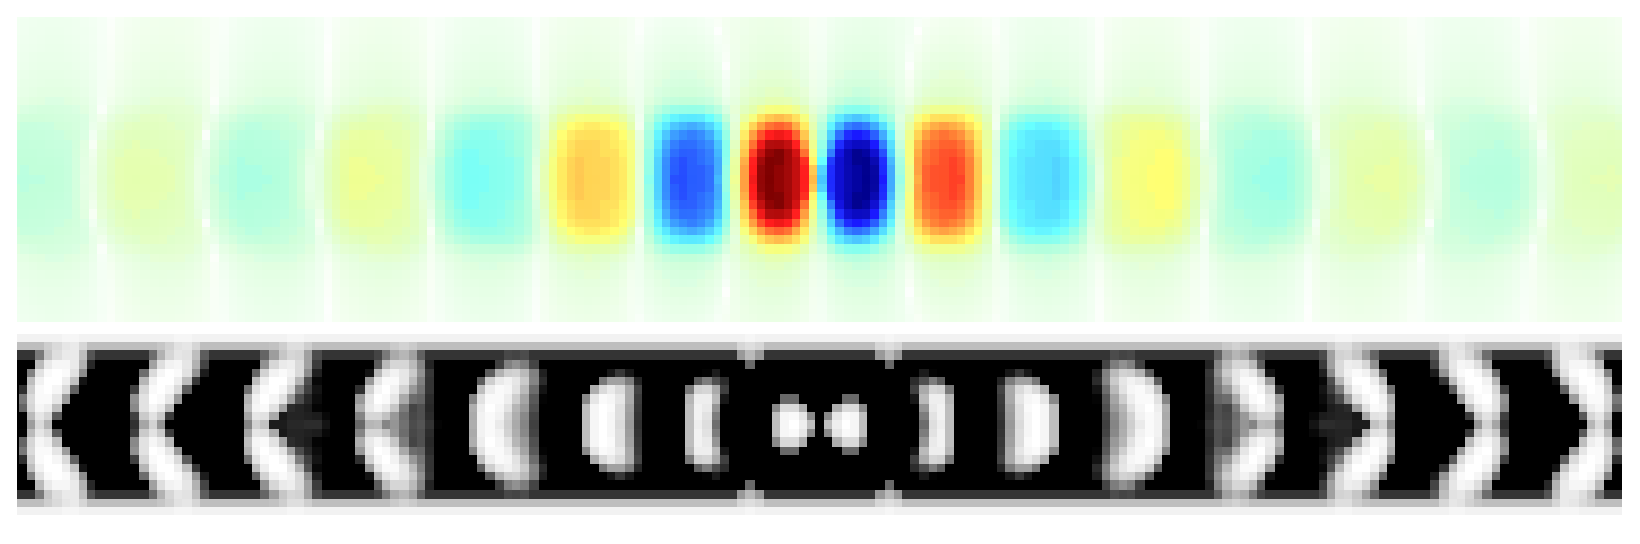
\includegraphics[width=1.0\textwidth]{fig2}
\caption{Magnetic field profile and two-dimensional dielectric structure of a small mode-volume resonator produced by our inverse design method.}
\end{figure}
	 

\end{document}

